\documentclass[twoside,a4paper]{article}

\usepackage{graphicx}
\usepackage{url}
\usepackage{listings}
\usepackage{color}

\definecolor{dkgreen}{rgb}{0,0.6,0}
\definecolor{gray}{rgb}{0.5,0.5,0.5}
\definecolor{mauve}{rgb}{0.58,0,0.82}

\lstdefinelanguage{Thicket}
{  
  morekeywords={
    adapter, module,from, import, export,
    type, enum, trait, model, class, 
    def, let, in, if, for, yield, 
    new, with
  },
  alsoother={-><?()},
  sensitive=true, % keywords are not case-sensitive
  morecomment=[l]{//}, % l is for line comment
  morecomment=[s]{/*}{*/}, % s is for start and end delimiter
  morestring=[b]" % defines that strings are enclosed in double quotes
}

\lstset{
  numbers=left,
  stepnumber=1,
  aboveskip=3mm,
  belowskip=3mm,
  showstringspaces=false,
  columns=flexible,
  basicstyle={\ttfamily},
  numberstyle=\tiny\color{gray},
  keywordstyle=\color{blue},
  commentstyle=\color{dkgreen},
  stringstyle=\color{mauve},
  breaklines=true,
  breakatwhitespace=false,
  tabsize=4
}

\lstset{language=Html}

\lstset{
 morekeywords={ adapter, module,from, import, export,
    typedef, type, trait, model, class, 
    def, let, in, if, for, yield, 
    new, with}
}

\lstset{
literate={~} {$\sim$}{1}
}

\usepackage[utf8]{inputenc}
% \usepackage[latin1]{inputenc}
\usepackage[T1]{fontenc}
\usepackage{actes}
\usepackage[french]{babel}
\title{ Du Web fonctionnel avec le langage Thicket }
\author{Didier Plaindoux$^1$}
% les titres de haut de pages
\titlehead{ Du Web fonctionnel avec le langage Thicket }%  a droite (page impaire)
\authorhead{Didier Plaindoux}% a gauche (page paire)
\affiliation{\begin{tabular}{rr} 
    \\ 1:  Fungus, Le village 31430 Gratens, France
    \\     {\tt d.plaindoux@fungus.fr}
\end{tabular}}

\begin{document}

\setcounter{page}{1}
\maketitle

\begin{abstract}
Nous pouvons  constater actuellement,  dans le monde  du développement
logiciel,   une  forte   adoption   du   paradigme  fonctionnel.   Les
applications  dites   Web  comptent  parmis  les   vecteurs  les  plus
importants pour la promotion de  cette approche. Ceci est notamment le
fait de langages fonctionnels fortement typés tels que Eml, Purescript
ou ScalaJS pour  ne citer qu’eux. Cependant ces  derniers reposent sur
un schéma  de compilation  procédant par  une “transpilation”  vers le
langage cible Javascript.

Cet article  court propose  d'aborder le  développement d'applications
clientes Web avec le langage  Thicket. Ce langage s’inscrit dans cette
mouvance des langages fonctionnels fortement  typés qui ciblent le Web
tout  en  y  intégrant  une  machine  virtuelle  spécifique  pour  son
exécution. Il dispose  de plus de constructions  syntaxiques dédiées à
la  dénotation  de  termes  HTML   afin  de  proposer  une  expression
déclarative de  la composition  de documents. Nous  verrons finalement
comment  ce langage  peut être  intégré  dans un  client. Cela  couvre
notamment le schéma  de compilation traditionnel mais  aussi un schéma
de compilation dit à la volée.
\end{abstract}

\section{Introduction}

Malgré l'existence  de langages  tels que  OCaml \cite{ocaml}  ou bien
Haskell \cite{haskell}, les principaux vecteurs de cet engouement sont
des  langages hybrides  comme  Scala \cite{scala}  ou bien  Java
\cite{java} avec son adoption des lambdas.

Cependant cet  engouement se trouve  aussi bien  porté par le  Web qui
accentue cette  mouvance. Ceci  est le  fait de  langages fonctionnels
fortement typés tels que  Eml \cite{elm}, Purescript \cite{purescript}
ou ScalaJS \cite{scalajs} pour ne citer qu’eux. Cependant ces derniers
reposent   sur   un   schéma   de  compilation   procédant   par   une
“transpilation” vers  le langage  cible Javascript. Malgré  les étapes
d’optimisation  mises  en  oeuvre  comme  par  exemple  le  traitement
spécifique  de la  recursion  terminale, une  telle transformation  ne
permet pas d’avoir une maitrise totale  du langage et de son exécution
comme  cela peut  être  le  cas avec  le  support  d’une machine  SECD
spécifique.

Cette dernière approche soulève cependant plusieurs problèmatiques. La
première  concerne l'expressivité  du langage  et notamment  lorsqu'il
s'agit de manipuler  le DOM \cite{dom}. En effet, a  l'instar de React
\cite{reacjs} ou Angular  \cite{angular2} qui sont centrés  sur le DOM
et sa manipulation,  la plupart des solutions  proposées procédent par
une  approche  fonctionnelle  des  balises HTML  rendant  de  ce  fait
difficile  la  conception.  Le  second  problème  concerne  le  modèle
d'éxécution qui  passe par la  plupart du temps par  une transpilation
vers Javascript.

Lors de l'élaboration  du langage Thicket ces  deux problèmatiques ont
été   particulièrement  ciblées   afin  d'étudier   l'expressivité  et
l'intégration dans le monde des applications dites Web.

\section{Survol très rapide du langage}

Thicket  est  un  langage  fonctionnel  fortement  typé  à  évaluation
paresseuse  intégrant  le  paradigme  objet par  l'apport  des  traits
\cite{trait}  et reposant  sur  un principe  de  séparation entre  les
classes et les modèles quelles dénotent.

Nous  proposons  un survol  très  rapide  du  langage en  couvrant  la
représentation des  données et  leur manipulation. Un  point important
concerne l'abscence d'effet de bord conférant au langage une propriété
dite d'immutabilité.  Ce dernier  point est important  notamment quand
sera abordé le cycle de vie d'une application dite Web.

\subsection{Modèle de données}

Une donnée  va être dénoté  par une expression de  type enregistrement
\cite{recordcalculus}.   Ainsi  toute   donnée  secondaire  est  alors
accessible  par le  nom associé.  Une données  est représentée  par un
ensemble d'attributs typés comme suit:

\lstset{language=Thicket}
\begin{lstlisting}
  model Personne {  
    nom: string   
    age: number
  }
\end{lstlisting}

Une générateur pour  le type {\tt Personne} est  alors synthétisé avec
une  signature  calquant  le  type   des  attributs  dans  l'ordre  de
spécification.   Construire une  donnée correspond  alors à  appliquer
cette  fonction.  Une  telle  définition n'est  pas  sans  oublier  la
définition  de   type  de  donnée  avec   enregistrements  en  Haskell
\cite{haskell}.

\lstset{language=Thicket}
\begin{lstlisting}
  Personne "Anakin Skywalker" 1 
\end{lstlisting}

De  cette donnée  il  est  alors aisé  d'extraire  une information  en
procédant par le nommage spécifique de la propriété souhaitée 
\footnote{Au  même  titre que  Scala  la  formulation  {\tt o  m}  est
  équivalement à {\tt o.m} dans le cadre d'utilisation des objets mais
  aussi des classes.}.

\lstset{language=Thicket}
\begin{lstlisting}
  (Personne "Anakin Skywalker" 1) nom
\end{lstlisting}

Le langage  repose aussi  sur la définition  de donnée  pouvants avoir
plusieurs  formes par  leurs énumération  au même  tire que  les types
injectifs  \cite{ocaml}   \cite{haskell}  ou  les  {\it   case  class}
\cite{scala}.   Par contre  le  filtrage de  forme  simple repose  sur
l'application de catamorphismes \cite{meijer1991functional} spécifiques.

\subsection{Manipulation des données}

Une classe  est un générateur  prenant en paramètre une  expression et
proposant en retour une base  de connaissance dans laquelle {\tt self}
dénote cette même  base.

\lstset{language=Thicket}
\begin{lstlisting}
  class jedi personne:Personne {
    nom: string
    grade: string
  } {
    def nom = personne.nom
    def grade = personne.age ?> 19 fold "Maitre" "Padawan"
  }
\end{lstlisting}

La création  d'une instance  de classe consiste  alors à  appliquer le
générateur associé.

\lstset{language=Thicket}
\begin{lstlisting}
  jedi (Personne "Anakin Skywalker" 1)
\end{lstlisting}

Finalement l'activation  d'une méthode consiste tout  simplement en un
envoi de message à l'instance.

\lstset{language=Thicket}
\begin{lstlisting}
  jedi (Personne "Anakin Skywalker" 1) grade
\end{lstlisting}

Cette  approche permet  de séparer  le modèle  du controlleur  ou plus
généralement le signifiant du signifier. Ce principe induit un système
avec lequel  plusieurs niveaux d'interpétation d'une  même donnée peut
être simplement élaboré.

\subsection{Immutabilité et système évolutif}

Un  des principes  de base  adopté lors  de l'élaborarion  du language
concerne  l'immutabilité. Pour  ce faire  toute donnée  est considérée
comme constante et ne peut donc être alors modifiée. L'unique approche
consiste à proposer  un système basé sur l'évolution de  donnée via un
jeu   de   fonctions   dites    anamorphiques   ou   de   {\em   lens}
\cite{meijer1991functional}.  Cette approche existe naturellement dans
les  langages  fonctionnels  comme  Haskell ou  OCaml  privé  du  {\tt
  mutable}.  Dans des langages récents comme Swift \cite{swift} il est
proposé la notion de structure pour  laquelle un objet peut évolué par
copie  partielle  impliquant  aussi   cette  notion  d'évolution  sans
modification de l'objet primaire.

Afin  de  faciliter l'expression  d'une  telle  transformation ll  est
possible de produire un nouvelle version de données par le biais d'une
structure de contrôle spécifique comme le montre le code qui suit.

\lstset{language=Thicket}
\begin{lstlisting}
  new Personne "Anakin Skywalker" 19 with nom = "Darth Vader"
\end{lstlisting}

Cette  même  structure  de  contrôle permet  aussi  d'opérér  sur  une
instance de  classe et  permettre ainsi  de faire  évoluer la  base de
connaissance d'une instance dans le temps.

\lstset{language=Thicket}
\begin{lstlisting}
  class jedi personne:Personne {
    nom: string
    grade: string
    anniversaire:  jedi
  } {
    def nom = personne nom
    def grade = personne age <? 21 fold "Padawan" "Maitre"
    def anniversaire = jedi new personne with age = (personne age + 1)
  }
\end{lstlisting}

Par le  biais de ce survol  rapide nous avons exposé  les principes de
bases  qui nous  ont conduit  à la  définition et  à l'élaboration  du
langage Thicket.  A  noter qu'il repose sur  des concepts parfaitement
maîtrisés concernant le typage mais aussi pour l'aspect fonctionnel.

\subsection{Cas de la manipulation du DOM}

Le point qui va nous intéresser maintenant concerne l'intégration d'un
tel langage dans  le monde des applications dites  Web.  Cela concerne
deux aspects. Le premier porte  sur la representation des données pour
le support HTML via le DOM  \cite{dom}. Dans la majorité des solutions
la mise en forme et la création de document sont prisent en charge par
des librairies fonctionnelles  pour la construction de  termes pour le
DOM \cite{dom}. 

Il existe  cependant une approche  déclarative - par opposition  à une
approche constructive -  permettant d'exprimer des fragments  et ce de
manière plus intuitive comme cela  est notamment le cas dans AngularJS
\cite{angularjs} et React \cite{react}.

\subsubsection{Expression de la structure d'un fragment}

Notre approche est sensiblement différente  car elle propose un modèle
d'expression qui est transformé en expression fonctionnelle lors de la
phase de  compilation. Une telle  approche permet de combiner  une vue
plus intuitive de la construction de document sans rompre le système.

\lstset{language=Thicket}
\begin{lstlisting}
  def vueJedi : jedi -> dom = j -> <p> j.grade " " j.nom </p> 
\end{lstlisting}

\noindent Bien  évidemment au même  titre que les langages  comme Elm,
Purescript   etc.    cette    expression   peut-être   remplacée   par
l'utilisation des librairies de la façon suivante:

\begin{lstlisting}
  def vueJedi : jedi -> dom = j -> {
      document "p" create addChild j.grade addChild " " addChild j.nom
  }
\end{lstlisting}

\subsubsection{Manipulation et système réactif}

Le deuxième  aspect de la  manipulation de DOM  concerne l'interaction
avec l'extérieur.   Dans notre approche  le comportement associé  à un
noeud du DOM est séparé de  la représentation.  Il devient alors ainsi
facile de  concevoir des  systèmes réactifs  par la  mise en  place de
points d'appels  permettant de  ce fait  d'appéhender la  structure du
document et des comportements associées.

\begin{lstlisting}
  def vueJedi : jedi -> dom = j -> {
    <p id="jedi"> j.grade " "  j.nom </p> 
    onMouseEvent MouseClick $ n -> console log "Click ..."
  }
\end{lstlisting}

La combinaison  de cette forme  réactive avec l'approche  évolutive va
nous  permettre  de  modéliser  simplement  les  applications  Web  en
proposant     une     approche    architecturale     unidirectionnelle
\cite{unidirectionnal} en  y intégrant  la réception et  le traitement
des interactions en  terme d'évolution de données  pour enfin terminer
par le rendu .
 
Dans note  exemple, ceci peut être  simplement mis en évidence  par la
combinaison  d'un  élément  visuel,  d'un capteur  d'évenement  et  la
fonction de traitement associée.

\begin{lstlisting}
  def vueJedi : jedi -> dom = j -> {
    <p id="jedi"> j.grade " "  j.nom </p> 
    onMouseEvent MouseClick $ _ -> documentRenderer <~ (vueJedi $ j anniversaire)
  }
\end{lstlisting}

\section{Une intégration Web sur mesure}

Afin de proposer un intégration fine  dans le monde du Web, la version
initiale du compilateur  a été ecrit en Javascript  contrairement à la
plupart  des   transpileurs  qui   sont  eux  en   Haskell  \cite{elm}
\cite{purescript}. Cette  approche nous  permet dès le  départ d'avoir
une prise  en charge  du langage  quasi-naturelle. Conjointement  à ce
choix le modèle  d'execution proposé ne repose pas  sur une traduction
du langage vers le langage cible à savoir Javascript pour le moment et
WebAssembly \cite{rossberg2016webassembly} plus  tard probablement. 

Concernant le  langage Thicket,  le choix est  bien au  contraire plus
traditionnel car le  code va dans un premier temps  - après les passes
de validations - être transformé en code objet. Ce même code est alors
pris en charge  par une machine de  Krivine \cite{krivine:2007}. Cette
approche offre  - comparativement à  la transpilation -  l'avantage de
découpler l'execution du  code de l'infrastructure qui  la porte. Cele
permet ainsi d'avoir une main mise totale sur le modèle d'exécution et
de l'outillage associé.

\subsection{Analyse, compilation à la volée et exécution}

En  terme  d'élaboration  d'application   le  code  source  peut  être
directement   embarqué   au   même   titre  qu'un   code   source   en
Javascript. Une  telle approche permet  d'avoir le même  apport qu'une
boucle d'évaluation  à savoir offrir un  prototypage rapide. Cependant
la contre-partie est  une compilation à la volée et  donc une phase de
validation pouvant lever des erreurs.

\lstset{language=Html}
\begin{lstlisting}
  <html lang="en">
  <head>
    <script type="application/thicket+package" data-src="Jedi"></script>
    <script type="application/thicket">
      from Jedi import vueJedi, jedi, Personne
      documentRenderer <~ $ vueJedi $ jedi $ Personne "Obi-Wan Kenobi" 1
    </script>

    <script src="/thicket/build/thicket-web-lang.min.js"></script>    
    <script type="application/javascript">
      function onLoad() { require('thicket')('/site').boot(); }
    </script>
  </head>        
    <body onload="onLoad()"> <div id="jedi"/> </body>
  </html>
\end{lstlisting}

Une application Web consiste dans  un premier temps à spécifier (ligne
3) le paquetages utilisés ainsi que  le programme à exécuter (lignes 5
et 6).  Pour la prise en charge du langage (ligne 9) le compilateur et
l'exécuteur sont  chargés et finalement quand  l'application est prête
l'analyse peut être enclenchée (ligne 11).

\begin{figure}[h]
\centering
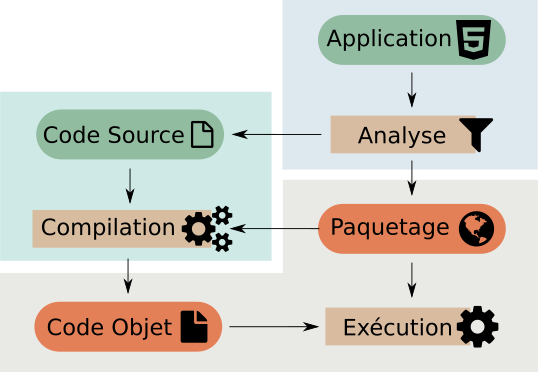
\includegraphics[scale=0.45]{repl} 
\caption{Schémas de compilation et execution}
\label{repl}
\end{figure}

L'exécution repose sur  trois phases. La première  consiste à analyser
le DOM pour la détection des paquetages à charger et les blocs de code
source à compiler et exécuter. Le seconde étape consiste à compiler et
charger  les  codes  objets  générés.  Finalement  la  dernière  étape
consiste à exécuter chacun des  code binaires à savoir les expressions
au  plus haut  niveau comme  celle ligne  6 de  notre exemple.  

La figure \ref{repl}  met en évidence une compilation dite  à la volée
mais  aussi  trois  étapes  clairement identifiée  avec  un  périmètre
délimité permettant de mettre en oeuvre  de bout en bout l'analyse, la
compilation  et l'exécution  du  code. 

\subsection{Analyse et exécution}

La modularisation mise en évidence  dans la figure \ref{repl} ouvre de
nouvelles perspectives comme  par exemple l'usage de  la compilation à
priori  comme  cela est  traditionnellement  mis  en oeuvre  pour  les
langages compilés.

Ainsi  la  phase d'analyse  peut  être  revisitée  afin de  mettre  en
évidence l'ensemble des code objets à exécuter.

\lstset{language=Html}
\begin{lstlisting}
  <html lang="en">
  <head>
    <script type="application/thicket+package" data-src="Jedi"></script>
    <script type="application/thicket+main" data-src="jedi.Main"></script>

    <script src="/thicket/build/thicket-web-runtime.min.js"></script>    
    <script type="application/javascript">
      function onLoad() { require('thicket')('/site').boot(); }
    </script>
  </head>        
    <body onload="onLoad()"> <div id="jedi"/> </body>
  </html>
\end{lstlisting}

La définition  passe non  seulement par la  phase de  spécification de
paquetages nécessaires pour la mise  oeuvre d'une application (line 3)
mais  aussi par  la mise  en  évidence des  codes à  exécuter lors  du
démarrage de l'application (ligne 4).

Le tout  est pris en  charge par  le module d'exécution  uniquement et
donc de la machine virtuelle associée.

\begin{figure}[h]
\centering
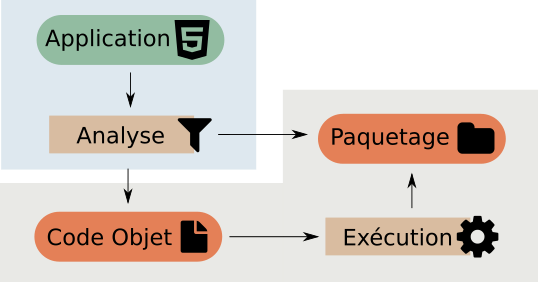
\includegraphics[scale=0.45]{execute} 
\caption{Schémas d'exécution}
\label{execute}
\end{figure}

\section{Perspectives}

De  ce premier  travail  il  en découle  un  ensemble de  perspectives
couvrant  le  domaine  de  la  compilation mais  aussi  le  domain  de
l'exécution.

\subsection{Compilation de document} 

Lors de  l'élaboration d'application l'injection de  code Thicket dans
toute page  HTML est pris  en charge dynamiquement. Cependant  lors du
passage  au  déploiement une  telle  technique  n'est pas  adaptée  et
peut-être couteuse. La  phase de compilation existante  dans un client
Web peut être alors reprise et  intégrée dans une phase de compilation
afin de  proposer une version  compilée et  donc optimale. Ce  type de
technique est  notamment appliquée  par des outils  d'assemblage comme
Bower \cite{bower} dans le monde du Web.

\subsection{Sécurisation du code}

Avec la maitrise de cette problèmatique d'execution et de distribution
l'aspect sécurité peut être entre autres revisité par la mise en place
de  système de  certification de  code objet  et de  paquetage par  la
signature.   

\subsection{Librairies spécifiques}

Bien  évidemment ces  deux derniers  aspects  ne sont  les seuls.   La
définition de librairies expressives doit permettre de mettre en place
des solution de type  unidirectionnelle \cite{unidirectionnal} pour la
gestion du cycle de vie d'une application par exemple.

\section{Conclusion}

Une  telle expérimentation  nous  permet d'explorer  non seulement  le
domaine des langages mais aussi chose aussi importante son intégration
dans des ecosystèmes distribués.  Cela couvre notamment la capacité du
language  à supporter  l'élaboration  d'application  dites riche  mais
aussi  le  mode  de  prise  en  charge  en  terme  d'execution  et  de
distribution à travers  le réseau par la gestion des  paquetages et de
leur distribution.

\bibliographystyle{abbrv}
\bibliography{mesreferences}

\end{document}
